% !TEX root = ../agglo_clust_review.tex

\section{Supplementary Material}

\begin{algorithm}
  \caption{\algname{} as a generalized edge contraction algorithm for signed graphs}
\hspace*{\algorithmicindent} \textbf{Input:} $\mathcal{G}(V,E,w^+,w^-)$ with $N$ nodes and $M$ edges; boolean \texttt{{\color{blue}addCannotLinkConstraints}} \\
\hspace*{\algorithmicindent} \textbf{Output:} Final clustering \\
  \hspace*{\algorithmicindent} 
  \begin{algorithmic}[1]
    % \Procedure{GraphEdgeContr}{{\color{blue}bool \emph{addConstraints}}}
      % \State $\mathcal{G}'\gets \mathcal{G}(V,E^+ \cup E^-)$ \Comment{Initialize the contracted graph}
      \State $\tilde{\mathcal{G}}(\tilde{V},\tilde{E}) \gets \mathcal{G}(V,E,w^+,w^-)$  \Comment{Init. contracted graph}
      \State \texttt{UF} $\gets$ initUnionFind($V$) \Comment{Init. data structure representing clustering}
    %   \State PQ $\gets$ Sort $e\in E$ in descending order of $|w_e|$
        \State PQ.push$(|w_e|, e) \quad \forall e \in E $  \Comment{Init. priority queue in desc. order of $|w_e|=|w_e^+ - w_e^-|$, $\mathcal{O}(|E|)$}
        \State \texttt{canBeMerged}$[e] \gets$ \texttt{True} $\,\,\, \forall e\in E$ \Comment{Init. cannot-link constraints}
      % \State $E_\dagger \gets \{\}$ \Comment{Set of must-not-link edges}
    %   \State PQ.push$(e,  ) \quad \forall e \in E $  
    \State
      \While{PQ is \textbf{not} empty}
        \State $\tilde{w}, e_{uv} \gets $ PQ.popHighest() \Comment{$\mathcal{O}(\log |E|)$}
        \State \textbf{assert} \texttt{UF}.find($u$) $\neq$ \texttt{UF}.find($v$) \Comment{Edges in PQ always link nodes in different clusters}
        % \If{ $e_{uv} \notin E' $} 
        %     \State \textbf{continue}
        % \EndIf
        \If{({\color{ForestGreen}\textbf{$\tilde{w} > 0$}}) \textbf{and} \texttt{canBeMerged}$[e_{uv}]$}
        %   \State $u,v \gets u,v \in V' : $
        %   \State $S_u \gets S \in \Pi$ : $ u \in S$
        %   \State $S_v \gets S \in \Pi$ : $ v \in S$
          \State PQ, \texttt{canBeMerged}, $\tilde{E}$ $\gets$ \textsc{UpdateNeighbors}($u,v$)
        %   \State mergeDoubleEdges($u,v$) \Comment{Update PQ, $E_\dagger, \mathcal{G}'$}
          
        %   \State Update costs of double edges;
        %   \State Propagate constrained flags of double edges;
          \State $\tilde{V} \gets \tilde{V} \setminus \{ v\}$, $\quad \tilde{E} \gets \tilde{E} \setminus \{ e_{uv}\}$ \Comment{Update contracted graph}
        %   \State $ S_u \gets S_u \cup S_v$
          \State \texttt{UF}.merge($u,v$) \Comment{Merge clusters, $\mathcal{O}(\alpha(|E|))$}
          % \For{every new double edge}
          %   \State Delete double edges
          %   \State Insert new one with updated cost
          % \EndFor
        \ElsIf{({\color{red}\textbf{$\tilde{\cost} \leq 0$}}) \textbf{and} {\color{blue}\texttt{addCannotLinkConstraints}}}
          \State \texttt{canBeMerged}$[e_{uv}] \gets$ \texttt{False} \Comment{Constrain the two clusters}
        \EndIf
      \EndWhile
      \State
    %   \State
      \Return Final clustering given by union-find data structure  \texttt{UF}
      % \State
    % \EndProcedure
  \end{algorithmic}
  \hspace*{1.5cm} 
    \begin{algorithmic}[1]
    \Function{UpdateNeighbors}{$u,v$}
      % \State $\mathcal{G}'\gets \mathcal{G}(V,E^+ \cup E^-)$ \Comment{Initialize the contracted graph}
      \State $\mathcal{N}_u = \{ t \in \tilde{V} | e_{ut}\in \tilde{E}  \}$
      \State $\mathcal{N}_v = \{ t \in \tilde{V} | e_{vt}\in \tilde{E}  \}$ 
      \For{$t \in \mathcal{N}_v$ } \Comment{Loop over neighbors in $\tilde{\mathcal{G}}$ of deleted node $v$}
        \State $\tilde{E} \gets \tilde{E} \setminus \{e_{vt}\}$
        \State $\tilde{w}_{vt} \gets$ PQ.delete($e_{vt}$) \Comment{$\mathcal{O}(\log |E|)$}
        \State \texttt{canBeMerged}$[e_{ut}] \gets$ \texttt{canBeMerged}$[e_{ut}]$ \textbf{and} \texttt{canBeMerged}$[e_{vt}]$
        \If{$t \in \mathcal{N}_u$ }\Comment{$t$ is a common neighbor of $u$ and $v$}
          \State $\tilde{w}_{ut} \gets$ PQ.delete($e_{ut}$)  \Comment{$\mathcal{O}(\log |E|)$}
          \State PQ.push($ |f(\tilde{w}_{ut}, \tilde{w}_{vt})|, e_{ut}$) \Comment{$\mathcal{O}(\log |E|)$  }
        % \EndIf
        \Else
          \State $\tilde{E} \gets \tilde{E} \cup \{e_{ut}\}$
          \State PQ.push($ |\tilde{w}_{vt}|, e_{ut}$) \Comment{$\mathcal{O}(\log |E|)$}
        \EndIf
      \EndFor
      \State
    %   \State
      \Return PQ, \texttt{canBeMerged}, $\tilde{E}$
    %   % \State
    \EndFunction
  \end{algorithmic}
  \label{detailed_alg}
  % \caption{where $\alpha$ is the slowly growing inverse Ackerman function}
\end{algorithm}
\begin{figure}
        \centering
\begin{minipage}{0.49\textwidth}
\centering
        % 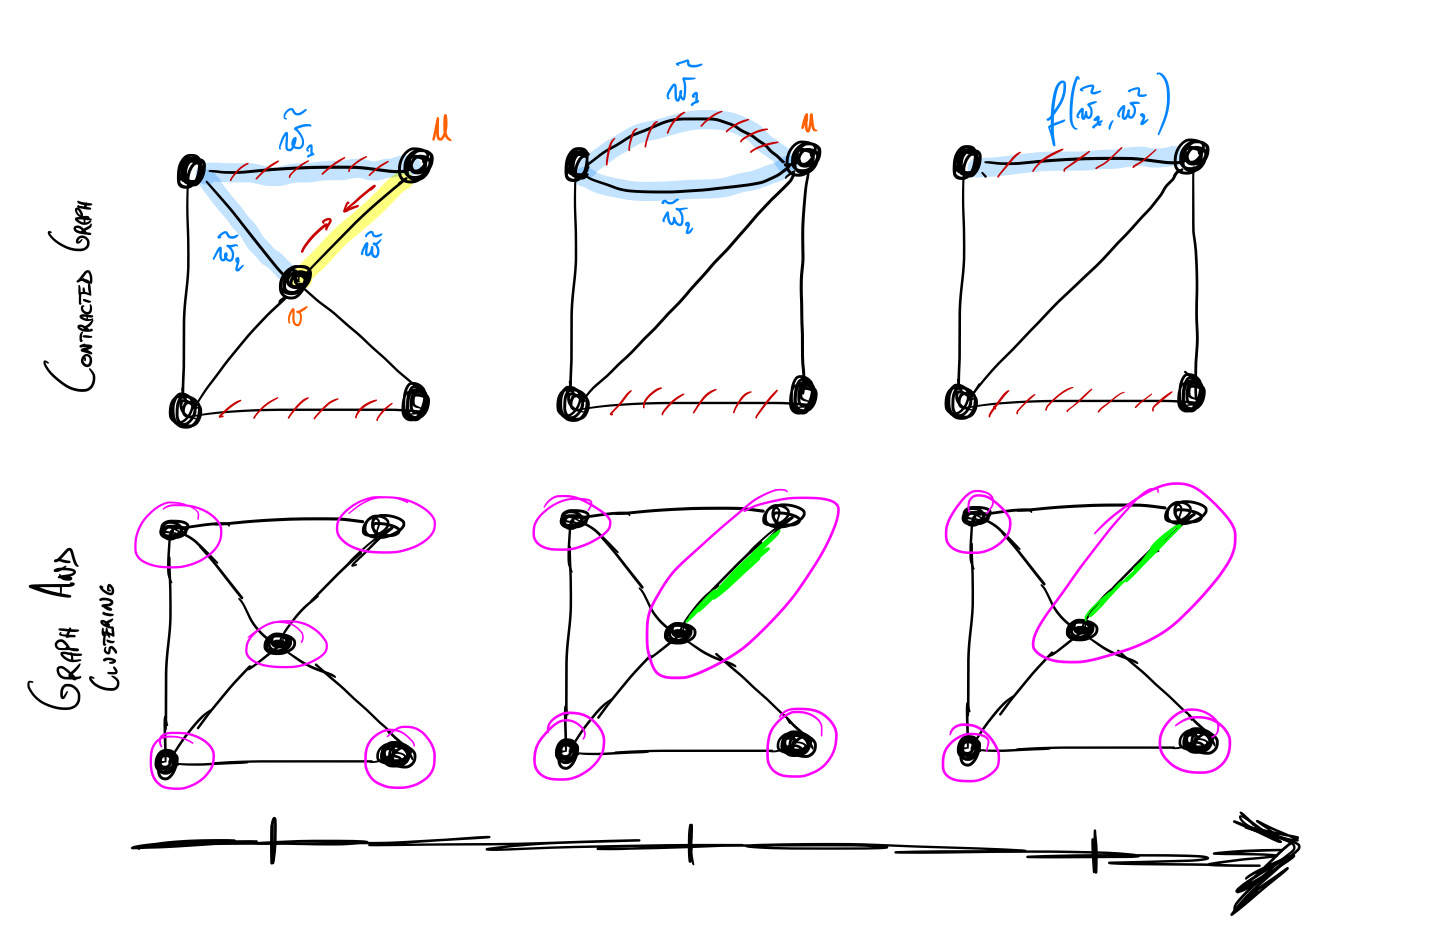
\includegraphics[width=\textwidth,trim=0.1in 0.4in 0.2in 0.2in,clip]{./figs/edge_contraction.png} % left bottom right top
        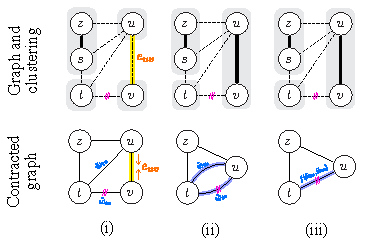
\includegraphics[width=\textwidth]{./figs/edge_contraction.pdf} % left bottom right top
% \captionof{figure}{ 
% {\small Example of edge contraction. First row: original graph $\mathcal{G}$; clustering $\Pi$ (gray shaded areas) with dashed edges on cut; cannot-link constraints (violet bars). Second row: contracted graph $\tilde{\mathcal{G}}_\Pi$. In step ii), edge $e_{uv}$ is contracted and node $v$ deleted from $\tilde{\mathcal{G}}_\Pi$. In step iii), double edges $e_{tu}$ and $e_{tv}$ resulting from edge contraction are replaced by single edge with updated interaction $f(\tilde{\cost}(e_{tu}), \tilde{\cost}(e_{tv}))$, see definitions in Tab.~\ref{tab:linkage-criteria}. }
% \label{fig:edge_contraction_and_contr_graph}  }
    \end{minipage} \hfill
\begin{minipage}[T]{0.48\textwidth}
    \centering
    \scriptsize
                \begin{tabular}[b]{r | l }
            \toprule
            % \multicolumn{2}{c||}{}  &   & \multicolumn{2}{c}{\textbf{Signed graphs}}  \\        
            % \cmidrule(l{.15em}){4-5}
            % \cline{4-5}
            % \multicolumn{2}{c||}{} & \textbf{Unsigned graphs} &  \multicolumn{2}{c}{\thead{Add Cannot-Link Constraints:}} \\        
            Linkage criteria & Update rule $f$ \\        
            \midrule
            Sum: & \thead[l]{$f(\tilde{\cost}_1,\tilde{\cost}_2) = \tilde{\cost}_1+\tilde{\cost}_2$} \\ 
            \makecell[r]{Absolute \\Maximum:} & \thead[l]{
            $
            f(\tilde{\cost}_1,\tilde{\cost}_2) = \begin{cases} 
            \tilde{\cost}_1 & \text{if}\,\, |\tilde{\cost}_1|>|\tilde{\cost}_2|\\
            \tilde{\cost}_2 & \text{otherwise}
             \end{cases} 
            $}
               \\ 
            \makecell[r]{Average:} & \thead[l]{$f(\tilde{\cost}_1,\tilde{\cost}_2) = \mathrm{weightAvg}\{ \tilde{\cost}_1, \tilde{\cost}_2 \} $}                 \\ 
            Maximum: & \thead[l]{$f(\tilde{\cost}_1,\tilde{\cost}_2) = \max \{ \tilde{\cost}_1, \tilde{\cost}_2 \}  $} \\
            Minimum:& \thead[l]{$f(\tilde{\cost}_1,\tilde{\cost}_2) = \min \{ \tilde{\cost}_1, \tilde{\cost}_2 \}  $} 
        \end{tabular}
    % \captionof{table}{}
    % \label{tab:linkage_and_update_rules}
\end{minipage}
\caption{ 
\textbf{Left:} Example of edge contraction. First row: original graph $\mathcal{G}$; clustering $\Pi$ (gray shaded areas) with dashed edges on cut; cannot-link constraints (violet bars). Second row: contracted graph $\tilde{\mathcal{G}}_\Pi$. In step ii), edge $e_{uv}$ is contracted and node $v$ deleted from $\tilde{\mathcal{G}}_\Pi$. In step iii), double edges $e_{tu}$ and $e_{tv}$ resulting from the edge contraction are replaced by a single edge with updated interaction. \textbf{Right:} The table lists the update rules $f(\tilde{\cost}_1, \tilde{\cost}_2)$ associated to the linkage criteria of Table \ref{tab:linkage-criteria} and that are used to efficiently update the interactions between clusters.}
\label{fig:edge_contraction_and_contr_graph}  
\end{figure}



\subsection{Implementation details and complexity of \algname{}} \label{sec:detailed_impl}


% During the agglomerative process, the interaction between adjacent clusters has to be properly updated and recomputed.  % given by the linkage criterion defined in Sec. \ref{sec:notation} and
% Given a graph $\mathcal{G}(V,E,\cost)$ and a clustering $\Pi$, we define the \emph{contracted graph} $\tilde{\mathcal{G}}_\Pi(\tilde{V}, \tilde{E}, \tilde{\cost})$, with $\tilde{V} \subseteq V$ such that node $u\in \tilde{V}$ represents the associated cluster $S_u \in \Pi$. Edges in $\tilde{E}$ are defined by adjacency-relationships between clusters and edge weights $\tilde{\cost}_{uv}$ represent inter-cluster interactions $\interact(S_u,S_v)$. 
\paragraph*{Update rules} During the agglomerative process, the interaction between adjacent clusters has to be properly updated and recomputed, as shown in Algorithm \ref{main_alg}.  % given by the linkage criterion defined in Sec. \ref{sec:notation} and
An efficient way of implementing these updates can be achieved by representing the agglomeration as a sequence of \emph{edge contractions} in the graph. Given a graph $\mathcal{G}(V,E,\cost)$ and a clustering $\Pi$, we define the associated \emph{contracted graph} $\tilde{\mathcal{G}}_\Pi(\tilde{V}, \tilde{E}, \tilde{\cost})$, such that there exists exactly one representative $|\tilde{V} \cap S| = 1$ for every cluster $S \in \Pi$ . Edges in $\tilde{E}$ represent adjacency-relationships between clusters 
and the signed edge weights $\tilde{\cost}_e$ are given by inter-cluster interactions $\tilde{\cost}(e_{uv})=\interact_{S_u,S_v}$. 
For the linkage criteria tested in this work, when two clusters $S_u$ and $S_v$ are merged, the interactions between the new cluster $S_u \cup S_v$ and each of its neighbors depend only on the previous interactions involving $S_u$ and $S_v$. Thus, we can recompute these interactions by using an \emph{update rule} $f$ that does not involve any loop over the edges of the original graph $\mathcal{G}$:
\begin{equation}
  \interact(S_u \cup S_v,S_t) = f\Big[ \interact(S_u,S_t), \interact(S_v,S_t) \Big] = f(\tilde{\cost}(e_{ut}), \tilde{\cost}(e_{vt})) %= \max \{ \tilde{\cost}(e_{ut}), \tilde{\cost}(e_{vt}) \}
\end{equation}
In Fig. \ref{fig:edge_contraction_and_contr_graph} we show an example of edge contraction and we list the update rules associated to the linkage criteria we introduced in Table \ref{tab:linkage-criteria}.
  % As an example, given the single-linkage criterion defined in Table , the interaction between $S_u \cup S_v$ and one of its neighbors $S_t$ is simply given by:
% All the update rules tested in this article are listed in Table \ref{tab:linkage-criteria}.

% \algname{} was implemented by using a standard agglomerative clustering algorithm based on a priority queue and a union
\paragraph{Implementation} As we show in Algorithm \ref{detailed_alg}, our implementation of \algname{} is based on an union-find data structure and a heap allowing deletion of its elements. The algorithm starts with each node assigned to its own cluster and sorts all edges $e\in E$ in a heap/priority queue (PQ) by their absolute weight $|\cost_e|=|w_e^+ - w_e^-|$ in descending order, so that the most attractive and the most repulsive interactions are processed first. It then iteratively pops one edge $e_{uv}$ from PQ and, depending on the priority $\tilde{\cost}_{uv}$, does the following: in case of attractive interaction $\tilde{\cost}_{uv}>0$, provided that $e_{uv}$ was not flagged as a cannot-link constraint, then merge the connected clusters, perform an edge contraction of $e_{uv}$ in $\tilde{\mathcal{G}}_\Pi$ and update the priorities of new double edges as explained in Fig. \ref{fig:edge_contraction_and_contr_graph}. 
% For every new pair of double edges in $\tilde{\mathcal{G}}_\Pi$, update their priorities according to one of the update rules listed in Table \ref{tab:linkage-criteria} together with their cannot-link relationships. 
If, on the other hand, the interaction is repulsive ($\tilde{\cost}_{uv}\leq 0$) and the option \texttt{addCannotLinkContraints} of Alg. \ref{detailed_alg} is \texttt{True}, then the edge $e_{uv}$ is flagged as cannot-link constraint.

\paragraph*{Complexity} In the main loop, the algorithm iterates over all edges, but the only iterations presenting a complexity different from $\mathcal{O}(1)$ are the ones involving a merge of two clusters, which are at most $N-1$. By using a union-find data structure (with path compression and union by rank) the time complexity of \texttt{merge}$(u, v)$ and \texttt{find}($u$) operations is $\mathcal{O}(\alpha(N))$, where $\alpha$ is the slowly growing inverse Ackerman function. The algorithm then iterates over the neighbors of the merged cluster (at most $N$) and updates/deletes values in the priority queue ($\mathcal{O}(\log |E|)$). Therefore, similarly to a heap-based implementation of hierarchical agglomerative clustering, our implementation of \algname{} has a complexity of $\mathcal{O}(N^2 \log N)$. In the worst case, when the graph is dense and $|E|=N^2$, the algorithm requires $\mathcal{O}(N^2)$ memory. Nevertheless, in our practical applications the graph is much sparser, so $\mathcal{O}(|E|)=\mathcal{O}(N)$. 
% and \UPDATE{in Fig. \ref{fig:runtime_plot} we show how the empirical runtime of \algname{} is much closer to $\mathcal{O}(N \log N)$ than $\mathcal{O}(N^2 \log N)$.} 
With a single-linkage, corresponding to the choice of the \emph{Maximum} update rule in our framework, the algorithm can be clearly implemented by using the more efficient Kruskal's Minimum Spanning Tree algorithm with complexity $\mathcal{O}(N \log N)$. 
Moreover, in the next section, we present an efficient implementation of \algname{} with \emph{Absolute Maximum} linkage that has empirical $\mathcal{O}(N \log N)$ complexity. %\TODO{Empirical complexity plot?}


\begin{algorithm}
  \caption{Mutex Watershed Algorithm proposed by \cite{wolf2018mutex}}
\hspace*{\algorithmicindent} \textbf{Input:} $\mathcal{G}(V,E,w^+,w^-)$ with $N$ nodes and $M$ edges \\
\hspace*{\algorithmicindent} \textbf{Output:} Final clustering \\
  \hspace*{\algorithmicindent} 
  \begin{algorithmic}[1]
      \State \texttt{UF} $\gets$ initUnionFind($V$) 
      % \State
      \For{$(u,v)=e\in E$ in descending order of $|w_e|=|w_e^+ - w_e^-|$}
        \If{\texttt{UF}.find($u$) $\neq$ \texttt{UF}.find($v$)} \Comment{Check if $u,v$ are already in the same cluster}
          \If{({\color{ForestGreen}\textbf{$w_e > 0$}}) \textbf{and} \texttt{canBeMerged}($u,v$)}  \Comment{Check for cannot-link constraints}
            \State \texttt{UF}.merge($u,v$) and inherit constraints of parent clusters
          \ElsIf{({\color{red}\textbf{$w_e \leq 0$}})}
            \State Add cannot-link constraints between parent clusters of $u,v$
          \EndIf
        \EndIf
      \EndFor
      \State
    %   \State
      \Return Final clustering given by union-find data structure \texttt{UF}
      % \State
    % \EndProcedure
  \end{algorithmic}
  \label{alg:mutex_watershed}
  % \caption{where $\alpha$ is the slowly growing inverse Ackerman function}
\end{algorithm}



\subsection{Properties of \algname{} with \emph{Absolute Maximum} linkage}\label{sec:appendix_abs_max}
\paragraph{Remark on graph notation} The definition of a graph proposed by \cite{wolf2018mutex} makes a distinction between a set of positive edges $E^+$, associated with a set $W^+$ of positive scalar attributes representing merge affinities, and a set of negative edges $E^-$, associated with a set $W^-$ of positive attributes representing split tendencies. On the other hand, in our definition $\mathcal{G}(V,E,w^+,w^-)$ each edge have both an attractive $w_e^+$ and a repulsive $w_e^-$ attribute, so we can make them equivalent by defining:
\begin{align}
E^+ = \{ e \in E \,\,\text{s.t.} \,\,w_e = w_e^+ - w_e^- > 0\},& \qquad E^- = \{ e \in E \,\,\text{s.t.}\,\, w_e = w_e^+ - w_e^- \leq 0\} \\
W^+ = \{ |w_e| \,\,\text{s.t.}\,\, e \in E^+\},& \qquad W^- = \{ |w_e| \,\,\text{s.t.}\,\, e \in E^-\}
\end{align}

\begin{prop} \label{prop:equiv_MWS}
The Mutex Watershed Algorithm \ref{alg:mutex_watershed} (MWS) with empirical $\mathcal{O}(N \log N)$ complexity introduced by \cite{wolf2018mutex} returns the same final clustering given by the \algname{} Algorithm \ref{detailed_alg} with the use of cannot-link constraints and an Absolute Maximum update rule:
\begin{equation}\label{eq:def_abs_max}
f_{\mathrm{Abs.Max.}}(\tilde{\cost}_1,\tilde{\cost}_2) = \begin{cases} 
            \tilde{\cost}_1 & \text{if}\,\, |\tilde{\cost}_1|>|\tilde{\cost}_2|\\
            \tilde{\cost}_2 & \text{otherwise}
             \end{cases} 
\end{equation}
\end{prop}
\begin{proof}
Both algorithms sort edges in descending order of the absolute interactions $|w_e|$ and then iterate over all of them. The only difference is that MWS, after merging two clusters, does not update the interactions between the new cluster and its neighbors. 
However, since with an Abs. Max. linkage the interaction between clusters is simply given by the edge with highest absolute weight $|w_e|$, the order by which edges are iterated over in \algname{} is never updated. Thus, both algorithms perform precisely the same steps and return the same clustering.
\end{proof}
\begin{prop}
The \algname{} Algorithm \ref{detailed_alg} with the Absolute Maximum linkage defined in Eq. \ref{eq:def_abs_max} returns the same final clustering whether or not cannot-link constraints are enforced. 
\end{prop}
\begin{proof}
% In Proposition \ref{prop:equiv_MWS} we observed that \algname{} with Abs. Max. linkage never updates the order by which edges are iterated over
In the \algname{} Algorithm \ref{detailed_alg}, the clustering is updated only when two clusters are merged and the condition at line 9 is satisfied. 
We also observe that, in the unconstrained version of \algname{}, the predicate \texttt{canBeMerged} at line 9 can never be false because cannot-link constraints are never introduced at line 14.
Let us now contradict the initial hypothesis and assume by absurd that the constrained version of \algname{} introduces a cannot-link constraints between two clusters sharing a positive interaction $\tilde{w}>0$ and outputs a different clustering as compared to the unconstrained version. 
This can happen only in the situation \TODO{shown in Fig. \ref{fig:contradiction_case}}, when two clusters $u$ and $v$ are merged together and share a common neighboring node $t$ having the following two properties: a) $u$ and $t$ are already constrained and share a repulsive interaction $w_{ut}\leq0$, b) $v$ and $t$ share an attractive interaction $w_{vt}>0$ that is higher in absolute value $|w_{vt}|>|w_{ut}|$. 
Then, according to Eq. \ref{eq:def_abs_max}, the new merged cluster $uv$ and $t$ are constrained and share a positive interaction. 
But this case can never happen, since if $|w_{vt}|>|w_{ut}|$ then clusters $v$ and $t$ are merged before clusters $u$ and $t$ are constrained.  
\end{proof}

% \subsection{Multicut and correlation clustering } 
% \TODO{Omit completely?} For any clustering $\Pi$ of $\mathcal{G}$, we define as $E^{\mathrm{internal}}_\Pi$ the set of edges linking nodes in the same cluster, and as $E_\Pi^{\mathrm{external}}$ the complementary set of edges whose incident nodes belong to distinct clusters:
% \begin{equation}
% E_\Pi^{\mathrm{internal}} \equiv \{ e_{uv} \in E \,|\, \exists S \in \Pi : u \in S \, \text{and} \, v \in S \}, \qquad E^{\mathrm{external}}_\Pi \equiv E \setminus E^{\mathrm{internal}}_\Pi.
% \end{equation}
% % \begin{align}
% % E_\Pi^0 &= \{ e_{uv} \in E \,|\, \exists S \in \Pi : u \in S \, \text{and} \, v \in S \}, \\
% % E^1_\Pi &= E \setminus E^0_\Pi.
% % \end{align}
% The set of edges $E_\Pi^{\mathrm{external}}$ is known as the \emph{multicut} of $\mathcal{G}$ w.r.t. clustering $\Pi$. The instance of the NP-hard \emph{weighted correlation clustering/multicut problem} 
% % w.r.t. $\mathcal{G}(V,E,\cost)$ 
% corresponds to finding the partitioning that optimally balance attraction and repulsion in the graph and is given by the following binary integer program \cite{kappes2011globally,chopra1991multiway,andres2015lifting}:
% \begin{equation}\label{eq:multicut_obj}
% % \min_\Pi \texttt{MC}(\Pi) \equiv
%  \min_\Pi \sum_{e\in E} \cost_e x_e^\Pi,  \qquad \text{where} \quad x^\Pi_e = 
%  \begin{cases} 
%  1 & \text{if } e\in E^{\mathrm{external}}_\Pi \\
%  0 & \text{otherwise}.
%  \end{cases}
% \end{equation}
% In the next chapters we will use this objective as measure of how balanced a clustering is.

\subsection{Predicting signed edge weights with a CNN}
Our CNN model outputs affinities in the form of pseudo-probabilities $p:E \rightarrow [0,1]$, where $p=0$ represents a boundary evidence. In order to use them as input of the algorithms in our framework, we mapped them to positive and negative values\footnote{Note that in general attractive and repulsive interactions $w^+$ and $w^-$ can be independently estimated with different classifiers.}. The most common approaches use \emph{additive} \cite{ailon2008aggregating} or \emph{logarithmic} \cite{finkel2008enforcing,andres2012globally} mappings:
\begin{equation} \label{eq:mappings}
\cost_{e,\mathrm{Add}} = p_e - \beta, \qquad \quad \cost_{e,\mathrm{Log}} = \log \left( \frac{p_e}{1-p_e} \right) - \log \left( \frac{\beta}{1-\beta} \right),
\end{equation}
where $\beta \in [0,1]$ is a \emph{bias} parameter that allow a tuning between over- and under-segmentation. We evaluated both of them empirically with each of the tested linkage and found that the additive mapping is the best option in all cases apart from the \emph{Sum} linkage. Note that varying the parameter $\beta$ does not usually define a hierarchy of nested clusterings, thus it is not equivalent to varying a threshold parameter in HAC. This hierarchical property is only valid for \algname{} without constraints and with \emph{Average}, \emph{Max} or \emph{Min} linkage.



\subsection{Neuron segmentation and compared methods}\label{sec:cremi_details}
\paragraph{Training details} The data from the CREMI challenge is highly anisotropic and contains artifacts like missing sections, staining precipitations and support film folds. 
To alleviate difficulties stemming from misalignment, we use a version of the data that was elastically realigned by the challenge organizers with the method of \cite{saalfeld2012elastic}.
We train a 3D U-Net \cite{ronneberger2015u, cciccek20163d} using the same architecture as \cite{funke2018large} and predict long-and-short range affinities 
as described in \cite{lee2017superhuman}. In addition to the standard data augmentation techniques of random rotations, random flips and  elastic deformations, we simulate data artifacts.
In more detail, we randomly zero-out slices, decrease the contrast of slices, simulate tears, introduce alignment jitter and paste artifacts extracted from the training data. Both \cite{funke2018large} and \cite{lee2017superhuman} have shown
that these kinds of augmentations can help to alleviate issues caused by EM-imaging artifacts.
We use L2 loss and Adam optimizer to train the network. % \TODO{Field of view?}

\paragraph{THRESH and WSDT} The basic post-processing methods we consider cannot take long-range affinities into account, so we only consider direct neighbors affinities and generate a boundary map by taking an average over the 3 directions. Based on this boundary map, we run connected components (THRESH) and we also introduce seeds at the maxima of the smoothed distance transform (WSDT). For WSDT, the degree of smoothing was optimized such that each region receives as few seeds as possible, without however causing severe under-segmentation. Due to the anisotropy of the data, we generate 2D WSDT superpixels by considering each 2D image in the stack singularly.


\paragraph{Multi-step pipelines} Given the 2D WSDT superpixels, we build a 3D region-adjacency graph such that each node represents a superpixel. The weights of the edges connecting neighboring superpixels are computed by taking an average over both short- and long-range affinities connecting the two regions. We then convert the edge probabilities to signed weights using the logarithmic mapping defined in Eq. \ref{eq:mappings} and solve the multicut problem on this graph. For our experiments, we use the approximate Kernighan-Lin solver \cite{keuper2015efficient,kernighan1970efficient} (WSDT+MC). In some cases, the long-range affinities predicted by the CNN can connect two superpixels that are not direct-neighbors. Thus, in these cases we introduce additional \emph{lifted} edges in the graph and an instance of the lifted multicut problem (WSDT+LMC). This time, similarly to the methods mentioned in \cite{beier2016efficient}, we used a combination of approximate solvers consisting in GAEC and Kernighan-Lin. 
%and      Other state-of-the-art multi-step-pipelines for neuron-segmentation first find 2D superpixels using WSDT and then apply a graph partitioning algorithm: in our comparison, we include one pipeline using hierarchical agglomerative clustering with average linkage (avgHC) and one using an approximation of the Lifted Multicut Problem (LMC) \cite{beier2016efficient}.

\subsection{\algname{} on the full CREMI dataset} \label{sec:appendix_exps_full_cremi}
 \paragraph{Pre-merge processing} For the predictions on the full dataset from the CREMI challenge, we used  the padded volumes provided by the challenge. The crops on which we performed a prediction have a size of $1500\times1500\times127=2.86\cdot 10^8$ voxels or larger. Building a graph with $10^8$ nodes can easily incur a large use of memory, so we decided to perform a preprocessing step by initially merging some nodes together. Simply down-sampling the predictions of the CNN would have led to a loss of resolution and performances in the most difficult parts of the dataset. Thus, we decided to pre-merge the most connected components of the graph that would be anyway clustered during the first iterations of \algname{}. To do this, we used a simple approach: we generated a boundary probability map by taking for each voxel an average over affinities in all directions (both short- and long-range ones) and we run THRESH to find the connected components. With this approach, pixels are pre-clustered only when they are far away (in all directions) from all predicted boundaries. 
 To make sure that in this preprocessing step different neurons are never merged together by mistake, we intersected these segments given by the conservative THRESH with the segments given by WSDT. %\TODO{show figure?}
 By using this method, we initialized \algname{} with a reduced graph that represents a true over-segmentation. In our experiments, the use of this preprocessing method did not impact the final scores achieved by \algname{} and significantly reduced its runtime. On the full datasets, we used only 10 \% of the long-range connections in the pixel-graph, since adding all of them did not improve the scores and only made the simulations much slower and memory inefficient. 
 
 \paragraph{Removing small segments} After running \algname{}, we use a simple post-processing step to delete small segments on the boundaries, most of which are given by single-voxel clusters. On the neuron segmentation predictions, we deleted all regions with less than 200 voxels and used a seeded watershed algorithm to expand the bigger segments.

 \paragraph{Enforcing local merge} In 2D images of urban-scenes, due to partial occlusion, one object instance can be given by multiple components that are not directly connected in the image plane. This is not the case in neuron-segmentation, where each neuron should be given by a single 3D connected component in the volume. In order to enforce it, we modified the implementation of \algname{} so that two clusters are merged only when they represent two adjacent supervoxels in the 3D volume and if this condition is not satisfied, the merge is postponed until there is a direct connection. This then avoids the introduction of ``air-bridges'' between segments due to attractive long-range connections in the initial voxel grid-graph.
 This approach achieved superior performances to the one proposed in \cite{wolf2018mutex}, where all long-range connections in the grid-graph are associated to a negative repulsive edge weight.

\begin{table}[t]
\centering
    \footnotesize
% \begin{minipage}[T]{0.85\textwidth}
%     \centering
        \begin{tabular}{l|c|c|c|c|c}
          \algname{} linkage & \makecell{Cremi-Score\\(higher better)}  & \makecell{Rand-Score\\(higher better)} & \makecell{VI-merge\\(lower better)} & \makecell{VI-split\\(lower better)} & \makecell{Runtime\\(lower better)} \\ \midrule
          % Pipeline & method & \textsc{No} & \textsc{Yes} \\ 

% Average & 0.226 & 0.936 & 0.315 & 0.494 & 
% Sum + CLC & 0.282 & 0.906 & 0.358 & 0.510 & 
% Abs Max & 0.322 & 0.897 & 0.286 & 0.735 & 
% Max + CLC & 0.324 & 0.893 & 0.292 & 0.698 & 
% Sum & 0.334 & 0.872 & 0.461 & 0.444 & 
% Average + CLC & 0.563 & 0.772 & 0.259 & 1.142 & 
% Min & 2.522 & 0.030 & 0.197 & 6.365 & 
% Min + CLC & 2.522 & 0.030 & 0.197 & 6.365 & 
% Max & 2.626 & 0.028 & 7.069 & 0.026 & 
Average & \textbf{0.226} & \textbf{0.936} & 0.315 & 0.494 & 3.49 $\cdot$ 10$^4$ \\
Sum + CLC \cite{levinkov2017comparative} & 0.282 & 0.906 & 0.358 & 0.510 & 4.64 $\cdot$ 10$^4$ \\
Abs Max \cite{wolf2018mutex} & 0.322 & 0.897 & 0.286 & 0.735 & 1.24 $\cdot$ 10$^4$ \\
Max + CLC & 0.324 & 0.893 & 0.292 & 0.698 & 6.31 $\cdot$ 10$^4$ \\
Sum \cite{keuper2015efficient} & 0.334 & 0.872 & 0.461 & 0.444 & 4.74 $\cdot$ 10$^4$ \\
Average + CLC & 0.563 & 0.772 & 0.259  & 1.142 & 2.95 $\cdot$ 10$^4$ \\
Min & 2.522 & 0.030 & \textbf{0.197} & 6.365 & 2.97 $\cdot$ 10$^3$ \\
Min + CLC & 2.522 & 0.030 & \textbf{0.197}  & 6.365 & 4.77 $\cdot$ 10$^3$ \\
Max & 2.626 & 0.028 & 7.069 & \textbf{0.026} & \textbf{6.04 $\cdot$ 10$^\mathbf{2}$} \\
        \end{tabular}
        \vspace*{1.1em}
    \caption{Performances achieved by different versions of \algname{} on the CREMI 2016 training set. CLC stands for cannot-link constraints. For all algorithms, the chosen value of bias parameter was $\beta = 0$.}
    \label{tab:extended_results_cremi}
\end{table}
% \hfill
% \begin{minipage}[T]{0.6\textwidth}
% \centering
%         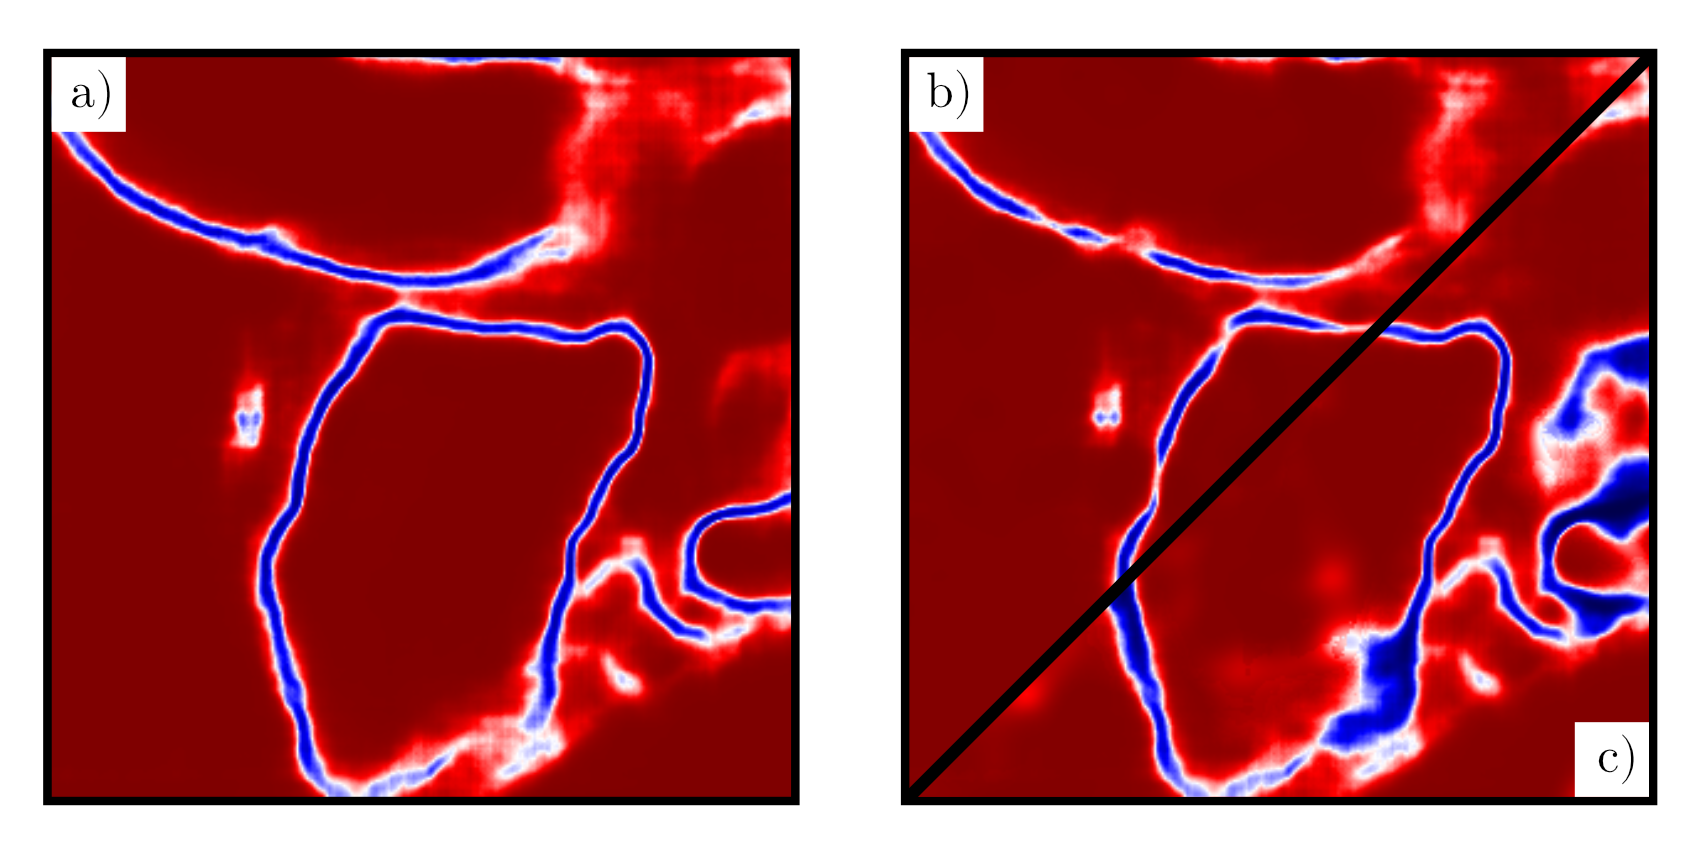
\includegraphics[width=0.88\textwidth,trim=0.1in 0.0in 0.05in 0.0in,clip]{figs/noisy_affs_comparison.png}
%     \captionof{figure}{The two figures represent the CNN predictions on a slice of the neuron segmentation CREMI challenge \cite{cremiChallenge} with and without additional noise. Blue pixels represent boundary evidence. Image a) shows the original CNN predictions, b) the merge-biased version $\tilde{F}_{+}$ and c) the split-biased version $\tilde{F}_{-}$ (see definition \ref{eq:noise_biased_predictions}). \TODO{Overlay raw-data}
%     %The color of each pixel represents how probable it is for it to be in the same cluster with its neighboring pixel on the right (red: same cluster; blue: different ones). 
%     %Adding merge-biased noise tends to create holes in the boundaries; split-biased noise add non-existing boundaries 
%     }
%     \label{fig:noisy_affs}
% \end{minipage}
% \end{figure}


\subsection{Experiments on neuron segmentation adding noise to CNN predictions} \label{sec:appendix_noise_gen}
Additionally to the comparison on the full training dataset, we performed additional experiments on a crop of the dataset\footnote{We chose a challenging part of CREMI training sample B}, where we perturbed the predictions of the CNN with noise and we introduced additional artifacts like missing or fictitious boundary evidences.
% Fig. \hyperref[fig:noisy_affs]{\ref*{fig:noisy_affs}a} shows an example of uncertain CNN predictions on a part of the neuron segmentation CREMI dataset. We now present a way of modifying the CNN output to introduce additional artifacts like a missing or false boundary evidence. 

In the field of image processing there are several ways of adding noise to an image, among which the most common are Gaussian noise or Poisson shot noise. 
In these cases, the noise of one pixel does not correlate with its neighboring noise values. On the other hand, predictions of a CNN are known to be spatially correlated. 
Thus, we used Perlin noise\footnote{In our experiments, we used an open-source implementation of simplex noise \cite{perlin2001noise}, which is an improved version of Perlin noise \cite{perlin1985image}}, one of the most common gradient noises used in procedural pattern generation. This type of noise $n(x)\in[0,1]$ generates spatial random patterns that are locally smooth but have large and diverse variations on bigger scales. We then combined it with the CNN predictions $p(x)$ in the two following ways: 
\begin{equation}\label{eq:noise_biased_predictions}
% \tilde{F}(x;\theta)=\begin{cases}
% F(x;\theta)+\mathcal{K}\cdot\max\left(N(x),0\right) & \text{if merge-biased}\\
% F(x;\theta)+\mathcal{K}\cdot\min\left(N(x),0\right) & \text{if split-biased}
% \end{cases}
\tilde{F}_{\pm}(x;\mathcal{K})=F(x)\pm\big|\mathcal{K}\cdot\max\left(\pm N(x),0\right)\big|,
\end{equation}
where  $N(x)=\mathrm{Logit}[n(x)]$; $F(x)=\mathrm{Logit}[p(x)]$ and $\mathcal{K}\in \mathbb{R}^+$ is a positive factor representing the amount of added noise. $\tilde{F}_{+}(x;\mathcal{K})$ represents then a under-clustering biased prediction, such that the probability for two pixels to be in the same cluster is increased only if $N(x)>0$ (see Fig. \hyperref[fig:noisy_affs]{\ref*{fig:noisy_affs}b}), whereas $\tilde{F}_{-}(x;\mathcal{K})$ is a over-clustering biased prediction with decreased probabilities when $N(x)<0$ (Fig. \hyperref[fig:noisy_affs]{\ref*{fig:noisy_affs}c}).
In the implementation we used, the noise can be generated in an arbitrary number of dimensions and a smoothing factor can be specified for each direction independently. In our experiments, each pixel is represented by a node in the grid-graph and it is linked to $n_{\mathrm{nb}}$ other nodes by short- and long-range edges. Thus, the output of our CNN model has $n_{\mathrm{nb}}$ channels: for each pixel / voxel, it outputs $n_{\mathrm{nb}}$ values representing the weights of different edge connections. We then generated a 4-dimensional noise that matches the dimension of the CNN output. The data is highly anisotropic, i.e. it has a lower resolution in one of the dimensions. Due to this fact, we chose different smoothing parameters to generate the noise in different directions. 

The experiments summarized in Fig. \ref{fig:noise_plots} were performed in the following way: for each value $\mathcal{K}$, 30 random noise samples were drawn, from which median and percentiles statistics were computed for each different linkage criteria. For each sample, we randomly selected some of the long-range predictions from the CNN and added them to pixel grid-graph.
% one of the dimensions has a lower resolution,   such that three dimensions represent the spatial ones a
% \multirow{2}{*}{Sum} &No & 0.55  & {\color{Orange} 0.313 } & {\color{Orange} 0.511 } \\
%  &Yes & 0.55  & {\color{Orange} 0.319 } & {\color{Orange} 0.527 } \\\midrule
% % Abs. max. &- & 0.45  & {\color{Orange} 0.321 } & {\color{ForestGreen} 0.531 } \\\midrule
% % \multirow{2}{*}{Mean} &No & 0.35  & {\color{ForestGreen} 0.343 } & {\color{ForestGreen} 0.552 } \\
%  % &Yes & 0.25  & {\color{Orange} 0.339 } & {\color{ForestGreen} 0.548 } \\\midrule
% \multirow{2}{*}{Max} &No & 0.85 & {\color{Red} 0.243 } & {\color{Red} 0.444 } \\
%  &Yes & 0.50  & {\color{Orange} 0.325 } & {\color{ForestGreen} 0.530 } \\\midrule
% \multirow{2}{*}{Min} &No & 0.50  & {\color{Red} 0.000 } & {\color{Red} 0.000 } \\
%  &Yes & 0.50  & {\color{Red} 0.000 } & {\color{Red} 0.000 } \\\midrule
% \cite{liu2018affinity} &-  & -  & {\color{ForestGreen} 0.341 } & {\color{ForestGreen} 0.547 } \\
\begin{figure}[t]
\centering
\begin{minipage}[T]{0.6\textwidth}
\centering
        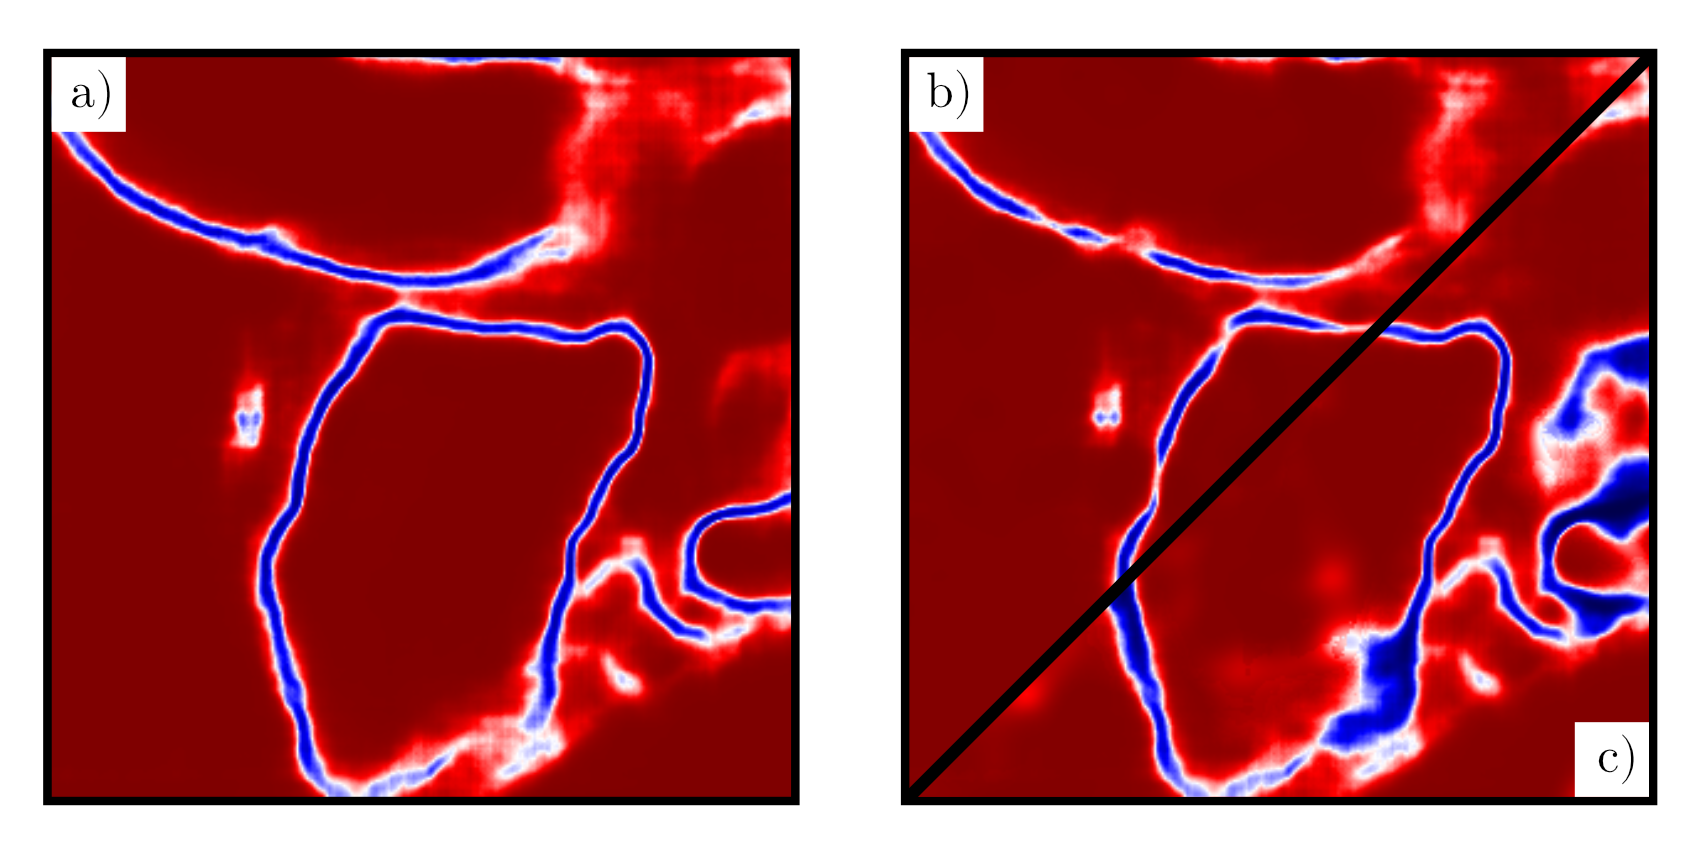
\includegraphics[width=0.88\textwidth,trim=0.1in 0.0in 0.05in 0.0in,clip]{figs/noisy_affs_comparison.png}
    \captionof{figure}{The two figures represent the CNN predictions on a slice of the neuron segmentation CREMI challenge \cite{cremiChallenge} with and without additional noise. Blue pixels represent boundary evidence. Image a) shows the original CNN predictions, b) the under-clustering biased version $\tilde{F}_{+}$ and c) the over-clustering biased version $\tilde{F}_{-}$ (see definition \ref{eq:noise_biased_predictions}). 
    %The color of each pixel represents how probable it is for it to be in the same cluster with its neighboring pixel on the right (red: same cluster; blue: different ones). 
    %Adding merge-biased noise tends to create holes in the boundaries; split-biased noise add non-existing boundaries 
    }
    \label{fig:noisy_affs}
\end{minipage}\hfill
\begin{minipage}[T]{0.35\textwidth}
    \centering
    \footnotesize
        \begin{tabular}{l|c|c}
          \algname{} linkage & AP  & Bias $\beta$ \\ \midrule
          % Pipeline & method & \textsc{No} & \textsc{Yes} \\ 
          Average & 34.3 & 0.35 \\
          Average + CLC & 33.9 & 0.25\\
          Max + CLC & 32.5 & 0.50 \\
          Abs Max & 32.1 & 0.45\\
          Sum + CLC & 31.9 & 0.55 \\
          Sum & 31.3 & 0.55 \\
          Max & 24.3 & 0.85 \\
          Min & 0.00 & 0.50 \\
          Min + CLC & 0.00 & 0.50 \\
        \end{tabular}
    \captionof{table}{Average Precision (AP) scores achieved by different versions of \algname{} and chosen bias parameters $\beta$ on the cityscapes validation set. A bias value $\beta=0$ returns one single cluster. CLC stands for cannot-link constraints}
    \label{tab:extended_results_cityscapes_val}
\end{minipage}
\end{figure}



\subsection{Fine-tuning the GMIS pipeline on CityScapes} \label{sec:appendix_cityscapes}
For our experiments, we used the model from GMIS \cite{liu2018affinity} that is publicly available. The instance-branch of the model was trained with a Binary Cross-Entropy loss, but we noticed how the short-range affinities were biased towards high probabilities, so that a strong short-range boundary evidence was never predicted by the model. In \cite{liu2018affinity}, they handle this problem by proposing a modified version of HAC that is done in stages (MultiStepHAC): initially only short-range affinities are used to run HAC and a low threshold in the hierarchy is chosen to define a first clustering; then a new HAC problem including long-range affinities is  initialized with the first clustering; in the method proposed by \cite{liu2018affinity}, these steps are repeated three times. 

Since MultiStepHAC is a rather complex post-processing method that requires to tune several hyper-parameters, we opted for a different approach to solve the problem of the unbalanced affinities. We added two 1x1 convolutional layers to the instance-branch model and trained them by using the same loss used for example by \cite{wolf2018mutex} and is based on the S\o resen-Dice coefficient \cite{dice1945measures,sorensen1948method}. Compared to Hamming-distance based loss like Binary Cross-Entropy or Mean Squared Error, the advantage of this loss is its being robust against prediction and / or target sparsity, that is a desirable quality in this application since boundaries between instances can be sparse. 
During training, all the affinities involving at least one pixel belonging to the background were ignored in the loss. In this way, these last two layers specialized in improving the predictions of boundary evidence between adjacent instances (especially those belonging to the same class). We then considered an average of these new fine-tuned affinities with the original unbalanced ones predicted by the model. During the fine-tuning process, only the parameters in the last two layers were updated.

Before to apply \algname{}, we performed a parameter-search for the bias $\beta$ defined in \ref{eq:mappings}. Table \ref{tab:extended_results_cityscapes_val} lists the best-case performances for each of the methods with the chosen bias $\beta$: note that depending on the version of \algname{}, it was necessary to bias more or less the predicted edge weights.


